%! Author = danielmendes
%! Date = 29.11.24

\chapter{Indexierung}\label{ch:indexing}

\section{Grundlagen}\label{sec:indexing-grundlagen}

Das folgende Thema befasst sich mit der Indexierung und den damit verbundenen Performance-Optimierungen, die näher erläutert werden.
Zunächst betrachten wir die Grundlagen der Indexierung, anschließend die verschiedenen Arten von Indizes und schließlich deren Auswirkungen auf die Performance.

Indizes sind Datenstrukturen, die von Speicher-Engines (engl. \ storage engines) verwendet werden, um unter anderem Zeilen schneller zu finden (\cite[pp. 147--189]{schwartz2012high}).
Sie haben einen großen Einfluss auf die Performance der Datenbank und werden umso wichtiger, je größer die Datenbank wird.
Weniger ausgelastete Datenbanken können ohne ordnungsgemäße Indizes gut funktionieren, aber die Leistung kann rapide sinken, wenn die Datenmenge wächst.
Wenn ein solches Problem auftritt, ist die Index-Optimierung oft der effektivste Weg, die Abfrageleistung zu verbessern.
Um wirklich optimale Indizes zu erstellen, ist es häufig notwendig, Abfragen umzuschreiben.
Wie genau Indizes erstellt werden müssen, wird im weiteren Verlauf der Arbeit betrachtet.

Um die Funktionsweise eines Indexes zu verdeutlichen, betrachten wir ein Beispiel aus einem wissenschaftlichen Fachbuch.
Am Ende solcher Bücher gibt es meist ein Stichwortverzeichnis oder Register.
Dieses Register besteht aus einer alphabetisch geordneten Liste von Begriffen, Themen und Stichworten.
Möchte man einen Begriff nachschlagen, sucht man ihn in der Liste und erhält die Seitenzahlen, auf denen er vorkommt.
In MySQL verwendet die Storage-Engine Indizes auf ähnliche Weise.
Sie durchsucht die Datenstruktur des Indexes nach einem Wert.
Wird ein Treffer gefunden, kann die Engine die Zeile ermitteln, die den Treffer enthält.
Betrachten wir dazu folgendes Beispiel:

\begin{lstlisting}[language=SQL,caption=Variationen,label={lst:select-query-customer}]
SELECT name FROM customer WHERE cust_id = 7;
\end{lstlisting}

Es gibt einen Index auf der Spalte \texttt{cust\_id}, sodass MySQL diesen Index nutzt, um Zeilen zu finden, deren \texttt{cust\_id} gleich 7 ist.
Mit anderen Worten wird eine Suche innerhalb der Indexwerte durchgeführt, und alle entsprechenden Zeilen werden zurückgegeben.

Ein Index kann Werte aus einer oder mehreren Spalten einer Tabelle enthalten.
Bei mehreren Spalten ist die Reihenfolge der Spalten im Index entscheidend, da MySQL nur effizient auf ein linkes Präfix des Indexes zugreifen kann.
Ein Index über zwei Spalten ist nicht gleichbedeutend mit zwei separaten einspaltigen Indizes.
Es gibt verschiedene Typen von Indizes, die jeweils für unterschiedliche Zwecke optimiert sind und die im nächsten Abschnitt behandelt werden.

Ein Index für ein bestimmtes Attribut A einer Tabelle ist eine Datenstruktur, die die Suche nach Tupeln mit einem bestimmen Wert für Attribut A effizienter macht (~\cite[pp. 350--353]{garcia2008database}).
Wenn Tabellen immer mehr Datensätze enthalten, wird es umso schwieriger alle Tupel zu scannen, um (nur wenige) Tupel zu finden, die zu einer Bedingung passen.
Besonders nützlich sind Indizes bei Abfragen, die Joins zwischen mehreren Tabellen enthalten, da sie ermöglichen, die Anzahl der zu prüfenden Tupel erheblich zu reduzieren, wenn eine einschränkende Bedingung vorliegt.

Datenbankmanagementsysteme ermöglichen das Erstellen von Indizes über mehrere Attribute.
Die Reihenfolge der Attribute ist hierbei entscheidend, da der Index nur effizient genutzt werden kann, wenn das erste Attribut der Reihenfolge in der Abfrage angegeben wird.
Gibt man nur das zweite Attribut an, ohne das erste zu referenzieren, kann der Index nicht direkt verwendet werden.

Das Auswählen von Indizes erfordert von den Entwicklern eine Tradeoff abzuwägen.
Es gibt dabei zwei Faktoren, die die Entscheidung beeinflussen.
Zum einen kann ein Index auf einem Attribut Abfragen mit diesem Attribut erheblich beschleunigen.
Zum anderen erschwert jeder Index Einfügungen, Löschungen und Aktualisierungen, da diese mehr Zeit und Aufwand erfordern.

Um zu verstehen, wie man Indizes für eine Datenbank auswählt, muss man wissen, wo bei der Bearbeitung einer Abfrage die meiste Zeit verbraucht wird.
Die Tupel einer Relation sind üblicherweise auf viele Seiten einer Festplatte verteilt, wobei eine Seite mehrere Tausend Bytes umfasst und viele Tupel speichert.
Um ein Tupel zu prüfen, muss die gesamte Seite, bzw.\ Block, in den Hauptspeicher geladen werden, wobei es kaum mehr Zeit kostet, alle Tupel einer Seite statt nur ein einzelnes zu prüfen.

Meistens ist der sinnvollste Index, den wir in einer Tabelle definieren können, der Schlüssel.
Das liegt zum einen daran, dass Abfragen auf diese Spalte sehr häufig vorkommen und zum anderen gibt es beim Schlüssel keine doppelten Werte, weshalb der Index entweder nichts oder genau eine Referenz auf ein Tupel zurückgibt.

Es gibt aber auch zwei Situationen, bei denen es hilfreich sein kann, einen Index auf Nichtschlüsselattribute zu definieren.
Zum einen wenn das Attribut ähnlich wie ein Schlüssel.
Damit ist gemeint, dass es für einen bestimmten Wert nicht genau ein Tupel gibt, wie bei einem Schlüssel, aber nur eine geringe Anzahl an Tupeln und damit werden auch weniger Festplattenzugriff für einen bestimmten Wert des Attributs benötigt wird.
Selbst wenn die Werte auf unterschiedlichen Blöcken gespeichert sind, sparen wir uns immer noch Zeit mit Index, wenn durch ihn nicht alle Blöcke geladen werden müssen.
Der andere Fall, bei dem ein Index sinnvoll sein könnte, wäre wenn die Tupel nach dem Attribut geclustert sind.
Das bedeutet, dass aufeinanderfolgende Ausprägungen des Attributs bei einem erstellten Index dazu führen, dass weniger Datenblöcke auf die Festplatte geladen werden müssen.

Jede Modifikation an einer Relation R zwingt uns dazu, jeden Index auf einem oder mehreren der modifizierten Attribute von R zu ändern.
Daher müssen wir nicht nur die Seiten von R lesen und schreiben, die modifiziert wurden, sondern auch bestimmte Seiten, die den Index enthalten, lesen und schreiben.
Aber selbst wenn Modifikationen die häufigste Form von Datenbankaktionen sind, kann es einen Effizienzgewinn bedeuten, einen Index auf ein häufig verwendetes Attribut zu erstellen.
Da tatsächlich einige Modifikationsbefehle Abfragen in der Datenbank beinhalten, muss man vorsichtig sein, wie man die relative Häufigkeit von Modifikationen und Abfragen schätzt.

Da eine Relation auf viele Festplattenblöcke verteilt ist, entstehen die Hauptkosten einer Abfrage oder Modifikation durch das Laden der Seiten in den Hauptspeicher.
Indizes können hierbei Zeit sparen, da sie den Zugriff auf Tupel ohne vollständige Durchsuchung der Relation ermöglichen.
Allerdings müssen auch Indizes auf der Festplatte gespeichert werden, was zusätzliche Festplattenzugriffe verursacht.
Modifikationen sind daher etwa doppelt so teuer wie der Zugriff auf den Index oder die Daten in einer Abfrage.

Um den neuen Wert eines Index zu berechnen, müssen wir Annahmen darüber treffen, welche Abfragen und Modifikationen mit hoher Wahrscheinlichkeit auf der Datenbank durchgeführt werden.
Manchmal haben wir eine Historie von Abfragen, die wir nutzen können, um gute Informationen zu erhalten, unter der Annahme, dass die Zukunft wie die Vergangenheit sein wird.

\begin{lstlisting}[caption=Deklaration der Beispieltabelle Fakten,label={lst:declaration-fakten}]
Fakten(Bestelldatum, Artikel_Id, Kunden_Id, ...)
\end{lstlisting}

\begin{lstlisting}[language=SQL,caption=1. Select-Query für Fakten,label={lst:fakten-select-query-kunden}]
SELECT Bestelldatum, Artikel_Id FROM Fakten WHERE Kunden_Id = k;
\end{lstlisting}

\begin{lstlisting}[language=SQL,caption=2. Select-Query für Fakten,label={lst:fakten-select-query-artikel}]
SELECT Bestelldatum, Kunden_Id FROM Fakten WHERE Artikel_Id = a;
\end{lstlisting}

\begin{lstlisting}[language=SQL,caption=Insert-Query für Fakten,label={lst:fakten-insert-query}]
INSERT INTO Fakten VALUES(d, a, k);
\end{lstlisting}

\begin{table}[h!]
    \centering
    \setlength{\arrayrulewidth}{0.4mm}
    \[
        \begin{array}{r|c c c c}
            \textbf{Aktion} & \textbf{Kein Index} & \textbf{Kunden Index} & \textbf{Artikel Index} & \textbf{Beide Indizes} \\ \hline
            Q_1 & 10 & 4 & 10 & 4 \\
            Q_2 & 10 & 10 & 4 & 4 \\
            I   & 2  & 4  & 4  & 6 \\ \hline
            \textbf{Durchschnitt} & 2 + 8p_1 + 8p_2 & 4 + 6p_2 & 4 + 6p_1 & 6-2p_1-2p_2 \\
        \end{array}
    \]
    \caption[Performance-Vergleich]{Darstellung der unterschiedlichen Queries mit Indexen}
    \label{tab:performance-queries}
\end{table}

\textbf{Voraussetzungen}
\begin{enumerate}
    \item Die \texttt{Fakten}-Tabelle belegt 10 Seiten, daher die Kosten bei gesamter Untersuchung bei 10.
    \item Im Durchschnitt kauft jeder Kunde kauft genau 3 Artikel und ein Artikel wird von 3 Kunden gekauft.
    \item Selbst mit Index gibt einen Durchschnitt von 3 Tupel für einen Kunden oder Artikel, ohne 10.
    \item Wenn eine Indexseite modifiziert/eingefügt werden muss, ist ein weiterer Festplattenzugriff erforderlich, um die modifizierte Seite zurückzuschreiben.
    \item Für eine Einfügung ohne Index sind auch zwei Festplattenzugriffe nötig.
\end{enumerate}

Wenn es nur einen Index auf Kunde gibt, erfordert Q2 immer noch einen Scan der gesamten Relation (Kosten 10).
Allerdings kann Q1 beantwortet werden, indem eine Indexseite gelesen wird, um die drei Tupel für einen bestimmten Kunden zu finden, und anschließend drei weitere Zugriffe erfolgen, um diese Tupel zu finden.
Einfügen I erfordert, dass sowohl eine Seite des Index als auch eine Seite der Daten gelesen und geschrieben wird, was insgesamt 4 Festplattenzugriffe bedeutet.

Die letzte Zeile in Abb.\ 8.3 gibt die durchschnittlichen Kosten einer Aktion an, unter der Annahme, dass der Anteil der Zeit, in der wir Qi ausführen, p1 beträgt und der Anteil der Zeit, in der wir Q2 ausführen, p2 ist.
Daher beträgt der Anteil der Zeit, in der wir I ausführen, 1 — p1 — p2.

Je nach pi und p2 kann jede der vier Optionen (Index/kein Index) die besten durchschnittlichen Kosten für die drei Aktionen ergeben.
Zum Beispiel, wenn pi = p2 = 0,1, dann ist der Ausdruck 2 + 8pi + 8p2 am kleinsten, sodass wir es bevorzugen würden, keine Indizes zu erstellen.

Das heißt, wenn wir überwiegend Einfügungen durchführen und nur sehr wenige Abfragen, dann wollen wir keinen Index.
Intuitiv, wenn wir viele Abfragen durchführen und die Anzahl der Abfragen, die Artikel und Kunden angeben, ungefähr gleich häufig sind, dann sind beide Indizes erwünscht.
Wenn wir nur ein Typ von Query häufig verwenden, dann sollten wir nur den Index definieren, der uns bei dieser hilft.

Das "Tuning" einer Datenbank umfasst nicht nur die Auswahl von Indizes, sondern auch die Festlegung vieler verschiedener Parameter.
Es gibt zahlreiche Tools, die entwickelt wurden, um diese Verantwortung vom Datenbankdesigner zu übernehmen, indem das System sich selbst optimiert oder dem Designer zumindest Empfehlungen für sinnvolle Entscheidungen gibt.
Dabei ermittelt das Tool zuerst die Abfragelast, dann können Einschränkungen festgelegt werden.
Anschließend werde Kandidaten-Indizes generiert und bewertet und zu guter Letzt wählt man die Index-Sets aus.
Ein komplexeres Problem tritt beim dritten Schritt auf, wenn bereits gewählte Indizes existieren, da diese beeinflussen können, wie viel Nutzen ein zusätzlicher Index bringt.
Ein bewährter Ansatz zur Auswahl von Indizes ist das sogenannte „greedy“-Verfahren, bei dem zunächst ohne ausgewählte Indizes der Nutzen jedes Kandidaten-Index bewertet wird.
Wenn es einen Index mit positivem Nutzen gibt, wird dieser ausgewählt und anschließend wird eine Neubewertung ausgeführt, wobei davon ausgegangen wird, dass der zuvor ausgewählte Index bereits verfügbar ist.
Dieser Prozess wird so lange wiederholt, bis es keinen Kandidaten-Index mit positivem Nutzen mehr gibt.

\section{B-Baum-Index}\label{sec:indexing-b-baum-index}

Indizes werden auf der Ebene der Storage-Engine und nicht auf der Serverebene implementiert.
Daher sind sie nicht standardisiert und unterscheiden sich je nach Engine.
Zudem unterstützen nicht alle Engines alle Indextypen.
Eine Storage-Engine ist eine Kernkomponente eines Datenbankmanagementsystems (DBMS), die für die Speicherung und Verwaltung der Daten zuständig ist.
Sie entscheidet, wie Daten physisch organisiert, gespeichert und abgerufen werden.
Verschiedene Storage-Engines unterscheiden sich in ihrer Indexfunktionalität sowie in der Unterstützung von Transaktionen und Sperrmechanismen.

Der erste zu betrachtende Indextyp ist der B-Baum-Index (engl. \ B-Tree Index), der auf einer speziellen Baum-Datenstruktur basiert.
Diese Struktur wird von den meisten MySQL-Storage-Engines unterstützt.
Die Implementierung und Nutzung des B-Baum-Indexes kann jedoch je nach verwendeter Storage-Engine variieren.

Das Grundprinzip eines B-Baums ist, dass alle Werte in einer bestimmten Reihenfolge gespeichert werden und jede Blattseite den gleichen Abstand zum Wurzelknoten hat.
Ein B-Baum-Index beschleunigt den Datenzugriff, da die Storage-Engine nicht die gesamte Tabelle durchsuchen muss, um die gewünschten Daten zu finden.
Stattdessen beginnt die Suche beim Wurzelknoten.

Die Slots im Wurzelknoten enthalten Zeiger auf Kindknoten, und die Storage-Engine folgt diesen Zeigern.
Der richtige Zeiger wird durch Vergleich der Werte in den Knoten-Seiten (engl. \ node pages) ermittelt, die die oberen und unteren Grenzen der Werte in den Kindknoten definieren.
Letztlich stellt die Storage-Engine fest, ob der gewünschte Wert existiert, oder sie erreicht erfolgreich eine Blattseite (engl. \ leaf page).

\begin{figure}[H]
    \centering
    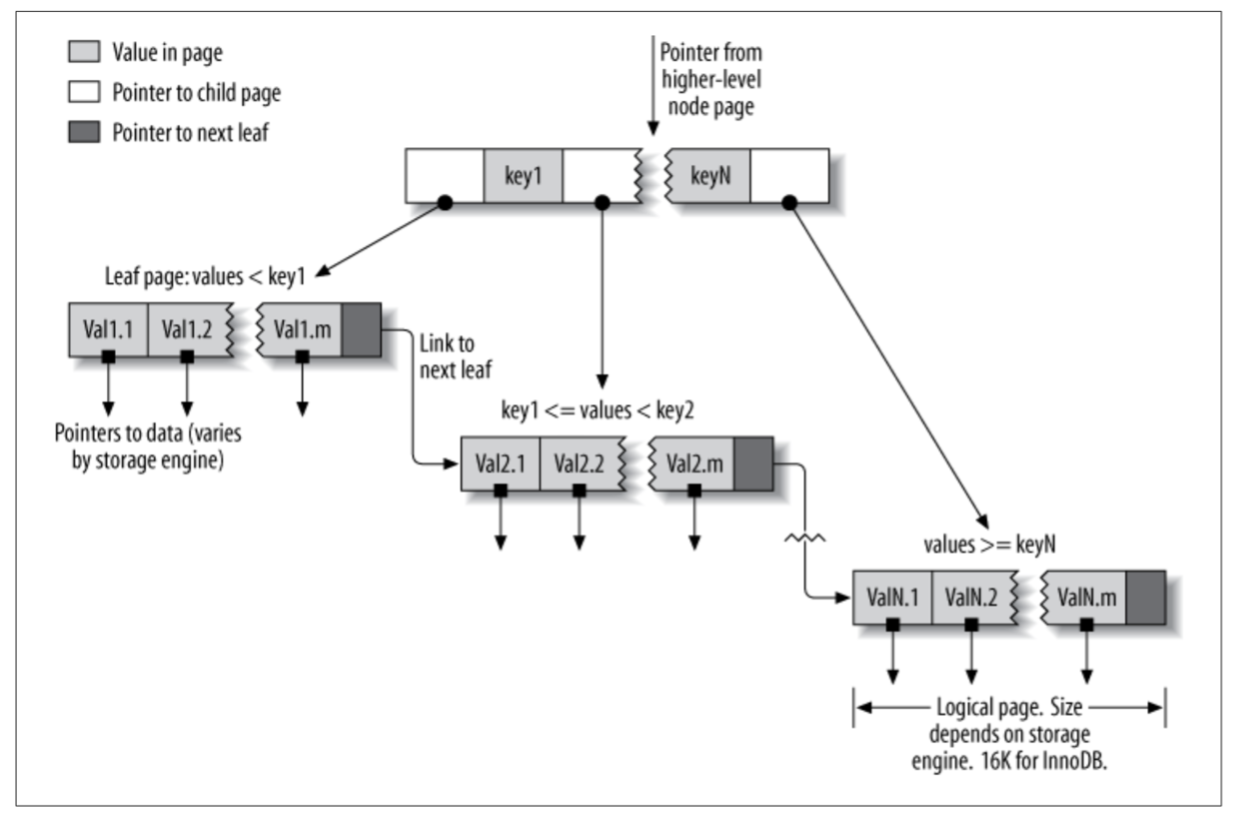
\includegraphics[width=0.8\textwidth]{PNGs/Textbook/B_Tree_Visualisation}
    \caption[Binärbaum-Visualisierung]{Darstellung des binären Baums mit Knoten und Blättern (Abbildung 5--1 aus \cite[S. 149]{schwartz2012high})}
    \label{fig:b-tree-visualisation}
\end{figure}

Blattseiten sind besonders, da sie Zeiger auf die indexierten Daten enthalten, anstatt auf andere Seiten zu verweisen.
Zwischen dem Wurzelknoten und den Blattseiten können viele Ebenen von Knoten-Seiten existieren.
Die Tiefe des Baumes hängt von der Größe der Tabelle ab.

Außerdem speichern B-Bäume die indexierten Spalten in einer festgelegten Reihenfolge, was sie besonders nützlich für die Suche nach Datenbereichen macht.
Beispielsweise kann ein Index auf einem Textfeld (z.B.\ vom Typ \texttt{VARCHAR}) effizient alle Namen finden, die mit „K“ beginnen, da die Werte in alphabetischer Reihenfolge gespeichert sind.

Der Index sortiert die Werte entsprechend der Reihenfolge der in der \texttt{CREATE TABLE}-Anweisung angegebenen Spalten, beispielsweise des Primärschlüssels (\texttt{last\_name, first\_name, b\_day}).
B-Baum-Indizes eignen sich gut für das Suchen mit dem vollständigen Schlüsselwert (engl. \ full key value), einem Schlüsselbereich (engl. \ key range) oder einem Schlüsselpräfix (engl. \ full key prefix).
Beim Schlüsselpräfix ist dies jedoch nur der Fall, wenn die Suche das linkeste Präfix des Indexes verwendet.

Als Nächstes betrachten wir die möglichen Abfragen, bei denen B-Baum-Indizes besonders hilfreich sind, um ein besseres Verständnis für ihre optimale Nutzung zu erlangen.
Eine Übereinstimmung mit dem vollständigen Schlüsselwert liefert Werte für alle Spalten im Index.
Eine beispielhafte Abfrage wäre die Suche nach allen Einträgen für Max Mustermann, geboren am 2000-01-01, wenn der Schlüssel aus Nachname, Vorname und Geburtsdatum besteht.
Für diesen Index sind auch Abfragen nützlich, die nur mit dem linken Präfix übereinstimmen, beispielsweise die Suche nach „Mustermann“.
Eine weitere Möglichkeit ist die Übereinstimmung mit einem Spaltenpräfix, also dem ersten Teil eines Spaltenwerts, etwa alle Nachnamen, die mit „M“ beginnen.
Ebenso effizient ist der Index bei der Übereinstimmung mit einem Wertebereich, z.B.\ Nachnamen zwischen „Mustermann“ und „Müller“.

Ein B-Baum-Index kann auch genutzt werden, um Abfragen effizient zu unterstützen, bei denen eine Spalte exakt und eine andere innerhalb eines Wertebereichs abgefragt wird.
Beispielsweise könnte dies eine exakte Übereinstimmung mit dem Nachnamen „Mustermann“ und eine Bereichsabfrage für Vornamen, die mit „Ma“ beginnen, umfassen.
Der letzte Anwendungsfall sind Abfragen, die nur den Index verwenden und nicht die gespeicherten Zeilen, etwa wenn alle benötigten Daten im Index enthalten sind.

Ein weiterer Vorteil von B-Baum-Indizes ist, dass sie aufgrund der sortierten Baumstruktur nicht nur Abfragen, sondern auch \texttt{ORDER BY}-Bedingungen effizient unterstützen können.
Wenn ein B-Baum für die Suche genutzt werden kann, kann er auch für die Sortierung der Ergebnisse verwendet werden.

Es gibt jedoch Einschränkungen von B-Baum-Indizes, die dazu führen, dass andere Indextypen für bestimmte Szenarien besser geeignet sind.
Eine Einschränkung ist, dass die Suche nicht am linken Ende des Indexes beginnen kann.
Beispielsweise ist ein Index, der aus Nachname, Vorname und Geburtsdatum besteht, nicht geeignet, um alle Personen zu finden, die vor dem Jahr 2000 geboren wurden, ohne dass der Nachname und Vorname ebenfalls spezifiziert werden.

Für optimale Leistung sollten Indizes mit den gleichen Spalten, jedoch in unterschiedlicher Reihenfolge erstellt werden, um die häufigsten Abfragen zu optimieren.
Eine Analyse der am häufigsten verwendeten Abfragen kann dabei helfen zu entscheiden, ob zusätzliche Indizes erforderlich sind.

Um die Benchmarks durchzuführen, erstellen wir zunächst wieder unsere Kundentabelle (\ref{lst:create_table_kunde}) und definieren folgende B-Tree-Indizes:

\vspace{-5pt}
\begin{lstlisting}[language=SQL,caption=Definition mehrere Indizes,label={lst:indexing-create-multiple}]
CREATE INDEX idx_stadt ON KUNDEN(STADT);
CREATE INDEX idx_postleitzahl ON KUNDEN(POSTLEITZAHL);
CREATE INDEX idx_geburtstag ON KUNDEN(GEBURTSTAG);
\end{lstlisting}
\vspace{-5pt}

Um die Effizienz dieser Indizes zu überprüfen, vergleichen wir diese Konfiguration mit einer, bei der nur die Kundentabelle und keine Indizes erstellt werden.
Anschließend werden in beiden Fälle eine bestimmte Anzahl an Datensätze eingefügt.
Um die Performance der Select-Abfragen zu messen, führen wir verschiedene Queries an die Datenbank aus, bei denen die Attribute \texttt{GEBURTSTAG}, \texttt{STADT} und \texttt{POSTLEITZAHL} berücksichtigt werden.
Dazu gehören \texttt{GROUP BY}- und \texttt{COUNT}-Abfragen, bei denen diese Attribute entweder direkt verwendet werden oder in der \texttt{WHERE}-Bedingung eine Rolle spielen.
Damit es übersichtlich genug bleibt, vergleichen wir 10 Datensätze mit 40 und 400 mit 4000 Zeilen.

\begin{figure}[H]
    \centering
    \begin{subfigure}[t]{0.48\textwidth}
        \centering
        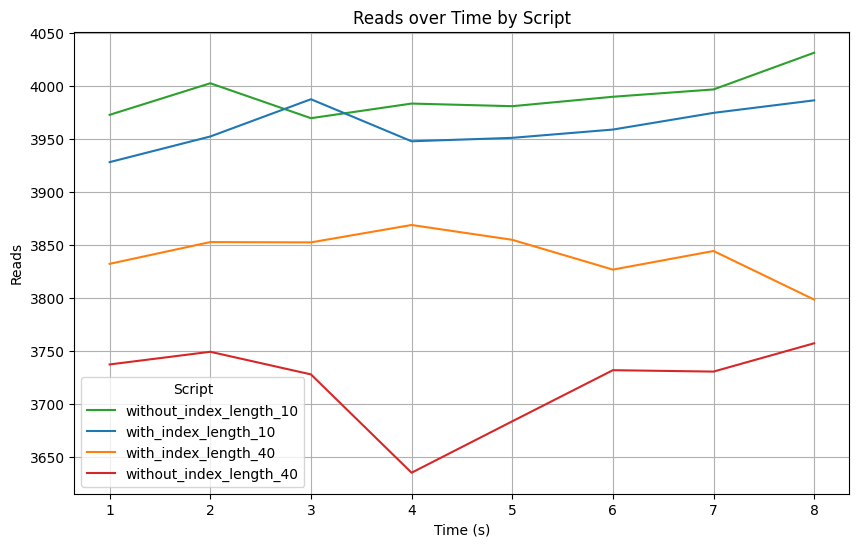
\includegraphics[width=\textwidth]{PNGs/Script/Index/B_Tree/low-count/Reads}
        \caption{Mit 10 und 40 Datensätze}
        \label{indexing-b-tree-low-reads}
    \end{subfigure}
    \hfill
    \begin{subfigure}[t]{0.48\textwidth}
        \centering
        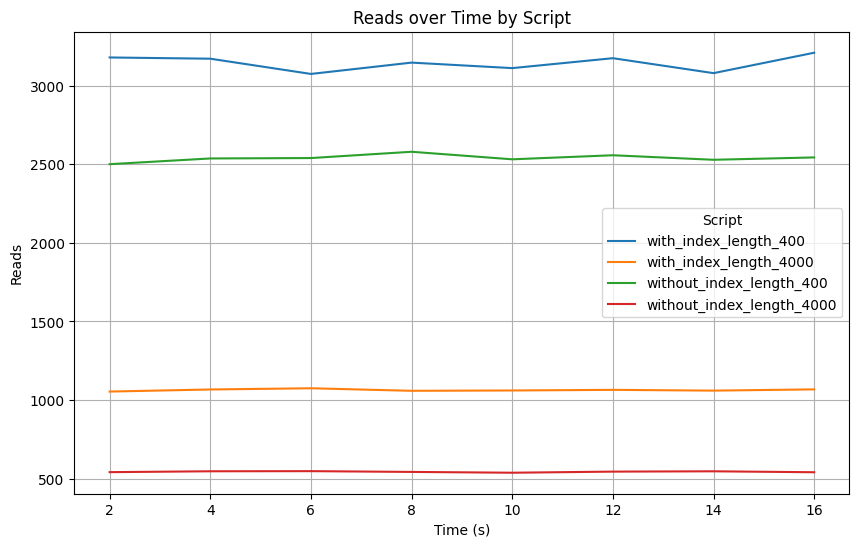
\includegraphics[width=\textwidth]{PNGs/Script/Index/B_Tree/high-count/Reads}
        \caption{Mit 400 und 4000 Zeilen}
        \label{indexing-b-tree-high-reads}
    \end{subfigure}
    \caption[B-Tree-Indexing: Mit Index vs Ohne]{Grafik zeigt Performance mit und ohne Index für Readsabfragen}
    \label{fig:indexing-vs-no}
\end{figure}
\vspace{-15pt}

In der Abbildung~\ref{indexing-b-tree-low-reads} können wir erkennen, dass bei 10 Datensätzen die Version ohne Indizes schneller ist als diejenige mit.
Bei 40, 400 oder 4000 (siehe~\ref{indexing-b-tree-high-reads}) Zeilen sehen wir aber schon die Wirkung, die die Indizes haben können, denn dort ist jeweils die Version mit Indizes effizienter.
Der Unterschied ist bei der Version mit 40 zwar etwas geringer, aber bei den anderen Fällen sehen einen deutlichen Unterschied.
Interessant ist, dass es nicht linear oder quadratisch mit der Anzahl an Datensätzen in der Tabelle steigt, sondern bei 400 und 4000 beträgt der Abstand jeweils etwa 500--700 ms.
Bei der Schreibgeschwindigkeit sind beide Versionen auf einem sehr ähnlichen Niveau, aber tendenziell hat die Version ohne Index einen leichten Vorteil.

Mit dem vorherigen Benchmark können wir die Vorteile eines Benchmarks schon deutlich erkennen.
Jetzt wollen wir aber auch die Wichtigkeit der richtigen Verwendung des B-Tree-Indexes untersuchen.
Dazu erstellen wir erneut die Kundentabelle, aber bestimmen dieses Mal nur einen Index.

\vspace{-5pt}
\begin{lstlisting}[language=SQL,caption=Definition für den 2. Benchmark,label={lst:indexing-create-single}]
CREATE INDEX combined_index ON KUNDEN(NAME, VORNAME, GEBURTSTAG);
\end{lstlisting}
\vspace{-5pt}

Wir befüllen die Tabelle mit einer festgelegten Anzahl an Datensätzen und führen unterschiedliche Select-Befehle aus.
Mit den verschiedenen Selects können wir erkennen, bei welchen Abfragen der Index am effizientesten ist.

\vspace{-5pt}
\begin{lstlisting}[language=SQL,caption=Unterschiedliche Where-Bedingungen für B-Tree-Index,label={lst:indexing-b-tree-selects}]
-- columm_prefix
WHERE NAME LIKE 'M%';
-- combined_match_with_range
WHERE NAME = 'Müller' AND VORNAME = 'Max' AND GEBURTSTAG < '1980-01-01';
-- exact_with_prefix
WHERE NAME = 'Müller' AND VORNAME LIKE 'M%' ORDER BY GEBURTSTAG;
-- full_match
WHERE NAME = 'Müller' AND VORNAME = 'Max' AND GEBURTSTAG = '1960-01-01';
-- leftmost_prefix
WHERE NAME = 'Müller';
-- not_leftmost
WHERE GEBURTSTAG < '1980-01-01';
-- range_values
WHERE NAME BETWEEN 'Müller' AND 'Schulz';
-- range_with_like
WHERE NAME = 'Müller' AND VORNAME LIKE 'M%' AND GEBURTSTAG < '1980-01-01';
-- skip_columns
WHERE NAME = 'Müller' AND GEBURTSTAG < '1980-01-01';
\end{lstlisting}
\vspace{-5pt}

Anhand der Grafik in Abbildung~\ref{fig:indexing-b-tree-query-reads} lässt sich erkennen, dass der \texttt{full\_match} die höchste Effizienz aufweist.
Es folgt \texttt{combined\_match\_with\_range}, bei dem die ersten beiden Argumente wie beim \texttt{full\_match} exakt bestimmt sind, während das dritte Argument, das Geburtsdatum, eine größere Flexibilität bietet, da hier alle Kunden berücksichtigt werden, die vor dem 01.\ Januar 1980 geboren wurden.
Im Anschluss kommt \texttt{range\_with\_like}, bei dem zusätzlich zum Geburtsdatum auch der Vorname mit "M" beginnen muss, jedoch nicht exakt "Max" sein muss.
Danach folgt \texttt{exact\_with\_prefix}, das dem vorherigen Fall ähnlich ist, jedoch zusätzlich eine aufsteigende Sortierung nach dem Geburtsdatum aufweist.
Dies zeigt, dass der B-Tree-Index auch für das Sortieren von Spalten genutzt werden kann.
Es folgt \texttt{skip\_columns}, bei dem der Vorname vollständig ignoriert wird.
Dadurch werden mehr Zeilen zurückgegeben, was die Performance negativ beeinflusst.
Anschließend kommt \texttt{leftmost\_prefix}, bei dem nur nach dem Namen gefiltert wird.
Bei \texttt{column\_prefix}, das direkt darauf folgt, wird statt des Namens „Müller“ jeder Nachname zurückgegeben, der mit „M“ beginnt.
Schließlich zeigt \texttt{range\_values} alle Namen zwischen „Müller“ und „Schulz“, während bei \texttt{not\_leftmost} ausschließlich nach dem Geburtsdatum gefiltert wird, ohne weitere Kriterien.
Insgesamt verdeutlicht diese Analyse die entscheidende Rolle des B-Tree-Index, da die Antwortzeiten je nach Art der Abfrage erheblich variieren können.

\begin{figure}[H]
    \centering
    \begin{subfigure}[t]{0.48\textwidth}
        \centering
        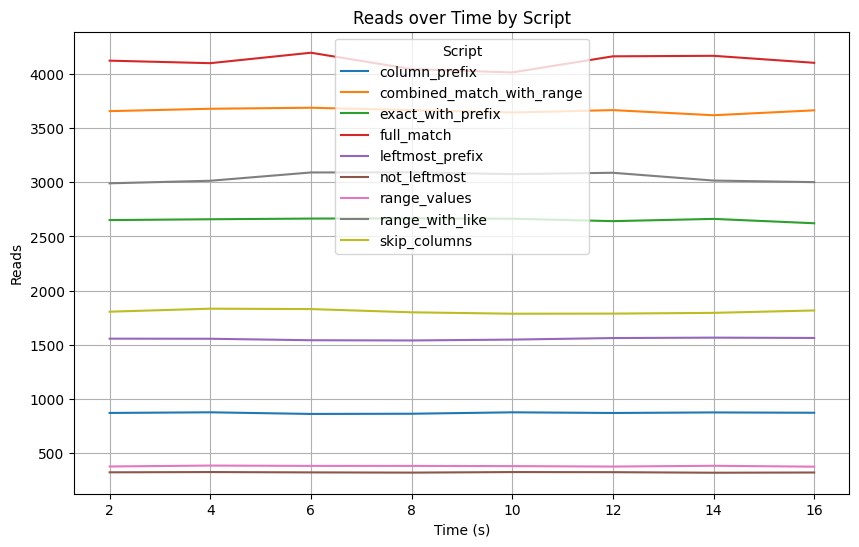
\includegraphics[width=\textwidth]{PNGs/Script/Index/B_Tree/b-tree-query-differences/Reads}
        \caption{Mit Index}
        \label{indexing-b-tree-query-reads-index}
    \end{subfigure}
    \hfill
    \begin{subfigure}[t]{0.48\textwidth}
        \centering
        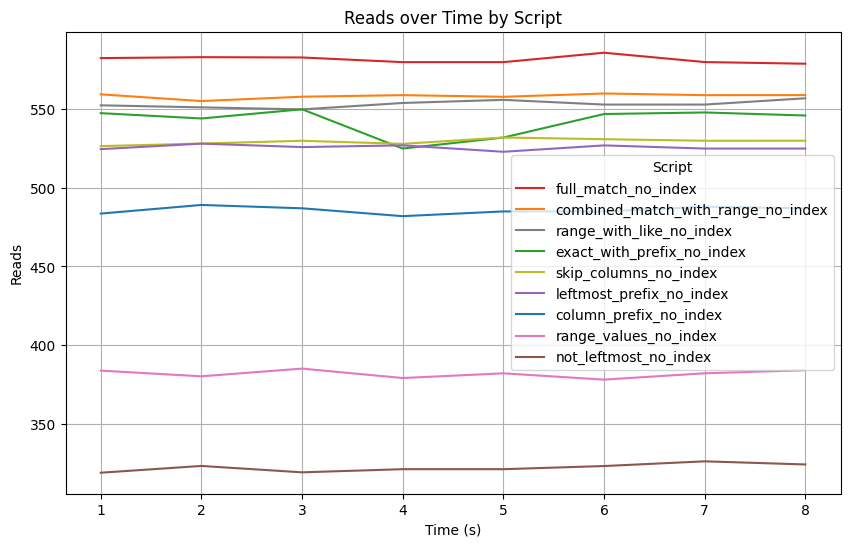
\includegraphics[width=\textwidth]{PNGs/Script/Index/B_Tree/b-tree-query-differences-no-index/Reads}
        \caption{Ohne Index}
        \label{indexing-b-tree-query-reads-no-index}
    \end{subfigure}
    \caption[B-Tree-Indexing: Unterschiedliche Selects mit Index und Ohne]{Visualisierung von unterschiedlichen Select-Queries mit und ohne Index}
    \label{fig:indexing-b-tree-query-reads}
\end{figure}
\vspace{-15pt}

Diese unterschiedlichen Zeiten hängen aber nicht nur davon ab, ob der Index verwendet werden kann, sondern auch wie viele Tupel jeweils zurückgegeben werden.
Wir können sehen, dass diejenigen Abfragen, die am wenigsten Zeilen zurückgeben, sind auch diejenigen sind, bei denen es die höchste Performance gibt.
Aber mithilfe des \texttt{EXPLAIN}-Operators können wir tatsächlich herausfinden, ob der definierte Index aus~\ref{lst:indexing-create-single} greift oder nicht.
Die Analyse von \texttt{EXPLAIN} zeigt, dass \texttt{range\_values} und \texttt{not\_leftmost} die einzigen sind, bei denen der Index nicht verwendet wird und beide sind auch die Langsamsten im Vergleich gewesen.

\begin{table}[H]
    \centering
    \begin{tabular}{|l|l|l|}
        \hline
        \textbf{Select-Query} & \textbf{Anzahl an Zeilen} & \textbf{Index benutzt?} \\
        \hline
        full\_match & 0 & ja \\
        combined\_match\_with\_range & 11 & ja \\
        range\_with\_like & 39 & ja \\
        exact\_with\_prefix & 65 & ja \\
        skip\_columns & 144 & ja \\
        leftmost\_prefix & 250 & ja \\
        column\_prefix & 509 & ja \\
        range\_values & 1313 & nein \\
        not\_leftmost & 2420 & nein \\
        \hline
    \end{tabular}
    \caption{Ergebnisse der COUNT(*)-Abfragen für B-Tree-Index}
    \label{tab:indexing_b_tree_count_results}
\end{table}
\vspace{-15pt}
TODO (Daniel): change the select-queries pls

\section{Hash-Index}\label{sec:indexing-hash-index}
Ein weiterer Indextyp, den wir betrachten, ist der Hash-Index.
Dieser basiert auf einer Hash-Tabelle und ist daher nur für exakte Suchanfragen geeignet, die alle Spalten im Index verwenden.
Die Funktionsweise der Storage-Engine lässt sich wie folgt beschreiben: Für jede Zeile wird mithilfe einer Hash-Funktion ein Hash-Wert der indexierten Spalte berechnet.
Der Hash-Wert (engl. \textit{hash code}) ist eine kleine Zahl, die sich in der Regel von den Hash-Werten anderer Zeilen mit unterschiedlichen Schlüsselwerten unterscheidet.

In MySQL unterstützt nur die Memory-Storage-Engine explizite Hash-Indizes.
Der bereits besprochene Standard-Indextyp für Memory-Tabellen, der B-Baum-Index, ist jedoch ebenfalls möglich.
Außerdem unterstützt die Memory-Engine keine eindeutigen Hash-Indizes.
Das bedeutet, wenn mehrere Werte denselben Hash-Wert besitzen, speichert der Index die Zeiger auf die Zeilen (engl. \textit{row pointers}) in demselben Hash-Tabelleneintrag, typischerweise mithilfe einer verketteten Liste (z.B.\ einer \textit{Linked List}).
Im Gegensatz dazu stellen eindeutige Hash-Indizes sicher, dass für jeden Hash-Wert nur ein einziger Eintrag existiert.
Bei Konflikten wird ein Mechanismus wie die \textit{Open Addressing}-Strategie (z.B. \textit{Linear Probing} oder \textit{Quadratic Probing}) eingesetzt, um Konflikte zu lösen und den Speicherplatz effizient zu verwalten.
Hierbei wird versucht, Konflikte direkt innerhalb der Hash-Tabelle zu bewältigen, anstatt auf zusätzliche Datenstrukturen wie verkettete Listen zurückzugreifen.

Um die Berechnung der Hash-Funktion genauer zu erläutern, folgt ein Beispiel:

\begin{lstlisting}[language=SQL,caption=Variationen,label={lst:select-query-hash}]
SELECT lname FROM testhash WHERE fname = 'Peter';
\end{lstlisting}

Zunächst berechnet MySQL den Hash-Wert für \texttt{'Peter'} und verwendet diesen, um den entsprechenden Zeiger im Index zu finden.
Angenommen, die Hash-Funktion liefert für \texttt{'Peter'} den Wert \textbf{7654}.
MySQL sucht nun im Index an der Position 7654 und findet einen Zeiger auf Zeile 3.
Im letzten Schritt wird der Wert in Zeile 3 mit \texttt{'Peter'} verglichen, um sicherzustellen, dass es sich um die richtige Zeile handelt.
Da die Indizes nur kompakte Hash-Werte speichern, sind Hash-Indizes äußerst platzsparend, und Suchvorgänge erfolgen in hoher Geschwindigkeit.

Ähnlich wie der B-Baum-Index hat auch der Hash-Index einige Einschränkungen, auf die wir nun eingehen:
Da der Index nur Hash-Werte und Zeiger auf Zeilen (engl. \textit{row pointers}) enthält, jedoch nicht die Werte selbst, kann MySQL den Index nicht verwenden, um das Einlesen der Zeilen zu vermeiden.
Da der Zugriff auf die in den Speicher geladenen Zeilen jedoch sehr schnell ist, wird die Leistung dadurch nicht wesentlich beeinträchtigt.

Ein wesentlicher Nachteil von Hash-Indizes ist, dass sie nicht für Sortierungen verwendet werden können, da die Werte nicht in einer geordneten Reihenfolge gespeichert sind.
Im Gegensatz dazu können B-Baum-Indizes Sortierungen unterstützen, wenn sie entsprechend erstellt und genutzt werden.
Darüber hinaus ermöglichen Hash-Indizes keine partiellen Schlüsselübereinstimmungen (engl. \textit{partial key matching}).
Da der Hash-Wert aus dem gesamten indexierten Wert berechnet wird, hilft ein Hash-Index beispielsweise nicht, wenn ein Index aus den Spalten (A, B) besteht und die \texttt{WHERE}-Klausel nur auf A verweist.
Ein weiterer Nachteil besteht darin, dass Hash-Indizes keine Bereichsabfragen (engl. \textit{range queries}) unterstützen.
Sie eignen sich lediglich für Gleichheitsvergleiche, wie die Operatoren \texttt{=} (gleich), \texttt{<=>} (null-sicher gleich) und \texttt{IN()}.

Obwohl Hash-Indizes sehr performant sind, können Hash-Kollisionen ihre Leistung beeinträchtigen.
Wenn viele Werte denselben Hash-Wert aufweisen, muss die Storage-Engine jeden Zeiger in der verketteten Liste durchlaufen und die entsprechenden Werte mit dem Suchwert vergleichen, um die richtige(n) Zeile(n) zu finden.
Auch Index-Wartungsoperationen können bei vielen Kollisionen langsamer werden.
Wenn beispielsweise ein Index auf einer Spalte mit sehr geringer Selektivität erstellt wird und eine Zeile gelöscht werden soll, kann das Finden des entsprechenden Zeigers im Index sehr aufwendig sein, was auch das Löschen der Zeile verzögert.

Einige Speicher-Engines, wie beispielsweise InnoDB, können zudem erkennen, wenn bestimmte Index-Werte besonders häufig verwendet werden, und automatisch einen Hash-Index für diese Werte im Speicher (engl. \textit{memory}) erstellen, der zusätzlich zu den vorhandenen B-Baum-Indizes genutzt wird.

Als Nächstes kommen wir zu den Benchmarks mit Hash-Indizes.
Dazu verwenden wir erneut die Kundentabelle und erstellen nur einen Index für die Spalte \texttt{NAME}.
Am Ende des \texttt{CREATE INDEX}-Befehl müssen wir \texttt{USING HASH} hinzufügen, damit anstelle des standartmäßigen B-Tree-Index der Hash-Index verwendet wird.
Danach befüllen wieder die Tabelle mit Testdaten.

Diesmal untersuchen wir beim ersten Benchmark den Einfluss von Hash-Kollisionen für die Performance.
Um den Grad der Kollisionen zu verändern haben wir eine Variable, die die obere Grenze für die zufällige Generierung einer Zahl, die an dem Namen herangehängt wird, darstellt.
Anschließend fragen wir alle Zeilen mit dem Wert \texttt{Kunde\_1} für die Spalte \texttt{NAME} ab.
Wir führen die Tests mit den Kollisionswahrscheinlichkeiten von 25\%, 10\%, 5\% und 1\% durch.

\begin{figure}[H]
    \centering
    \begin{subfigure}[t]{0.48\textwidth}
        \centering
        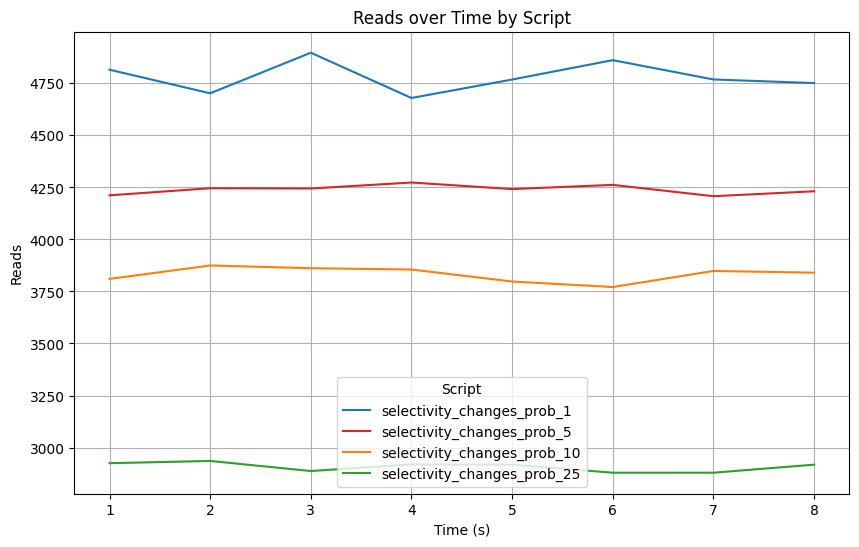
\includegraphics[width=\textwidth]{PNGs/Script/Index/Hash/selectivity-change/Reads}
        \caption{Unterschiede von Readsabfragen}
        \label{hash-collision-reads}
    \end{subfigure}
    \hfill
    \begin{subfigure}[t]{0.48\textwidth}
        \centering
        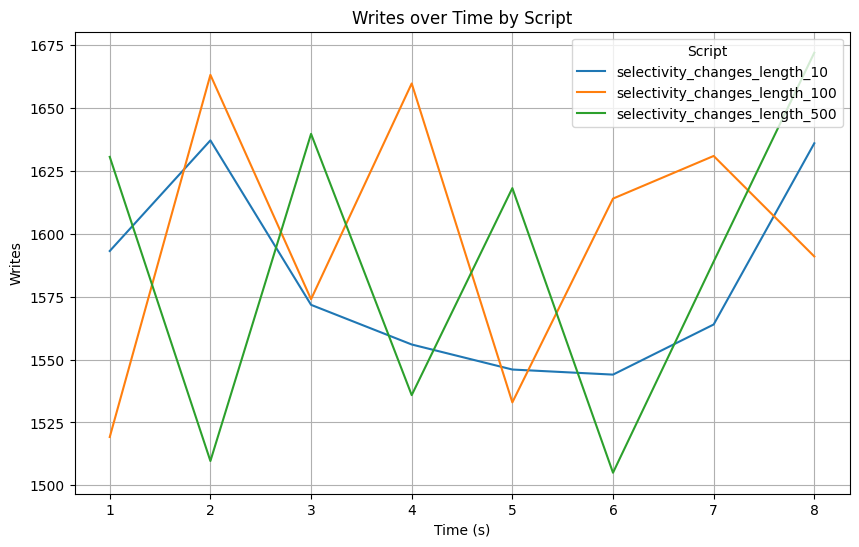
\includegraphics[width=\textwidth]{PNGs/Script/Index/Hash/selectivity-change/Writes}
        \caption{Unterschiede von Schreibbefehlen}
        \label{hash-collision-writes}
    \end{subfigure}
    \caption[Hash-Indexing: Auswirkungen von Hashkollisionen]{Vergleich der Auswirkungen von Hashkollisionen}
    \label{fig:hash-collision-comparison}
\end{figure}
\vspace{-15pt}

An den Ergebnissen in Abbildung~\ref{fig:hash-collision-comparison} können wir sehen, dass je geringer die Wahrscheinlichkeit für eine Kollision ist, desto schneller ist die Select-Abfrage.
Es fällt auch auf, dass die Unterschiede zwischen den verschiedenen Kollisionswahrscheinlichkeiten sehr groß sind.
Hingegen die Einfüge-Performance ist überraschenderweise bei allen 4 Varianten auf einem ähnlichen Niveau.

Als zweiten Test wollen wir wieder überprüfen, ob der Index bei bestimmten Select-Queries benutzt wird oder nicht.
Wie erwartbar benutzen wir wieder unsere Kundentabelle und erstellen den gleichen Index wie in Beispiel~\ref{lst:indexing-create-single}.
Anschließend fügen wir wieder die Testdaten ein und verwenden wieder die Select-Befehle aus~\ref{lst:indexing-b-tree-selects}.
Dieses Mal benutzen wir aber nicht alle Select-Befehle, sondern nur die folgenden:

\begin{table}[H]
    \centering
    \begin{tabular}{|l|l|l|}
        \hline
        \textbf{Select-Query} & \textbf{Anzahl an Zeilen} & \textbf{Index benutzt?} \\
        \hline
        full\_match & 0 & ja \\
        combined\_match\_with\_range & 4 & nein \\
        exact\_with\_prefix & 41 & nein \\
        leftmost\_prefix & 201 & nein \\
        \hline
    \end{tabular}
    \caption{Ergebnisse der COUNT(*)-Abfragen für Hash-Index}
    \label{tab:indexing_hash_count_results}
\end{table}
\vspace{-15pt}

Wie schon aus der Tabelle~\ref{tab:indexing_hash_count_results} ersichtlich wird, wir nur bei \texttt{full\_match} der Index verwendet.
Diese Erkenntnis können wir auch aus dem Result des Benchmarks (siehe~\ref{fig:indexing-hash-query-readsh}) erkennen.
Denn die Query ist um ein Erhebliches schneller als alle anderen (etwa um Faktor 15).
Alle anderes Queries sind sehr ähnlich, was unter anderem auch der Skalierung geschuldet ist.
Obwohl \texttt{combined\_match\_with\_range} nur 4 Zeilen zurückgibt und \texttt{leftmost\_prefix} hingegen 201 Datensätze, sind die Unterschiede nur sehr klein.

\begin{figure}[H]
    \centering
    \begin{subfigure}[t]{0.48\textwidth}
        \centering
        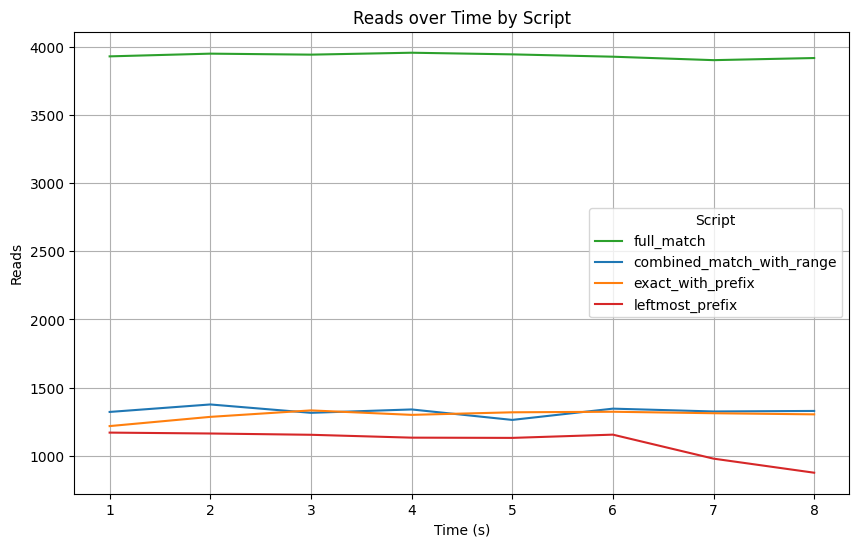
\includegraphics[width=\textwidth]{PNGs/Script/Index/Hash/hash-query-differences/Reads}
        \caption{Mit Index}
        \label{indexing-hash-query-reads-index}
    \end{subfigure}
    \hfill
    \begin{subfigure}[t]{0.48\textwidth}
        \centering
        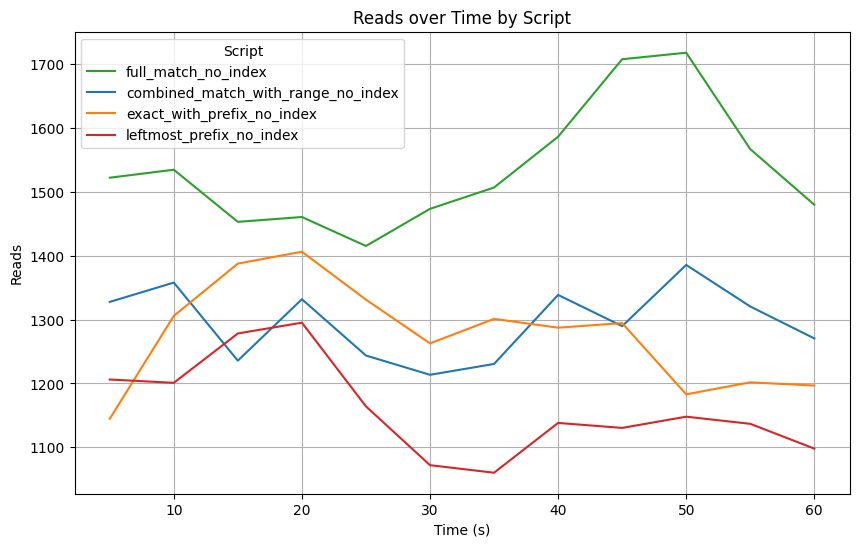
\includegraphics[width=\textwidth]{PNGs/Script/Index/Hash/hash-query-differences-no-index/Reads}
        \caption{Ohne Index}
        \label{indexing-hash-query-reads-no-index}
    \end{subfigure}
    \caption[Hash-Indexing: Unterschiedliche Abfragen mit Index und Ohne]{Grafik visualisiert unterschiedlichen Select-Queries mit und ohne Index}
    \label{fig:indexing-hash-query-reads}
\end{figure}
\vspace{-15pt}